%"###############################################
%
% Classification RTUPB pre 
%
%###############################################

\begin{figure}[H]
\centering
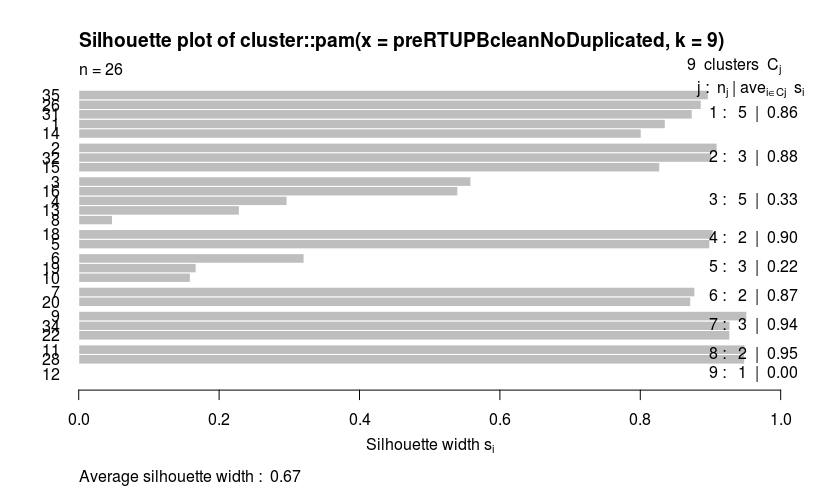
\includegraphics[width=0.90\textwidth]{../Fig/RTUPB/rtupb-silpam-pre}
\caption{Maximise nb cluster / bonne classification}
\end{figure}

Si nous cherchons la valeur qui maximise Nombre cluster/bons classements. ici nous avons avons deux resultats possibles en 
concurrence à savoir deux clusters. 
Ici il est interressant de voir dés le deuxieme cluster nous avons un classement qui semble pertinent. Au regard de la silouhette 
il apparrait que nous avons selement 3 individus dans un cluster ceux ci hormis l'age ont presque  les memes valeurs. En observant la courbe  nous avons un autre candidat à partir d'une segmentation en 9 clusters. 

\begin{figure}[h]
\centering
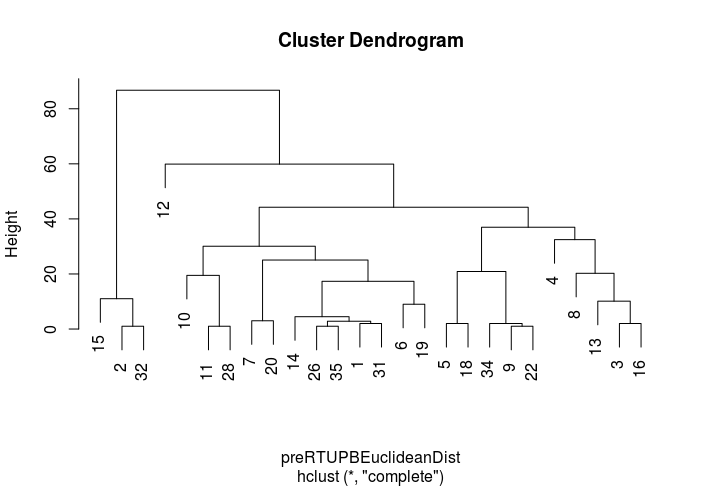
\includegraphics[width=0.90\textwidth]{../Fig/RTUPB/rtupb-cah-empty.png}
\caption{Moyenne silouhette }
\end{figure}

La CAH 


\begin{figure}[H]
\centering
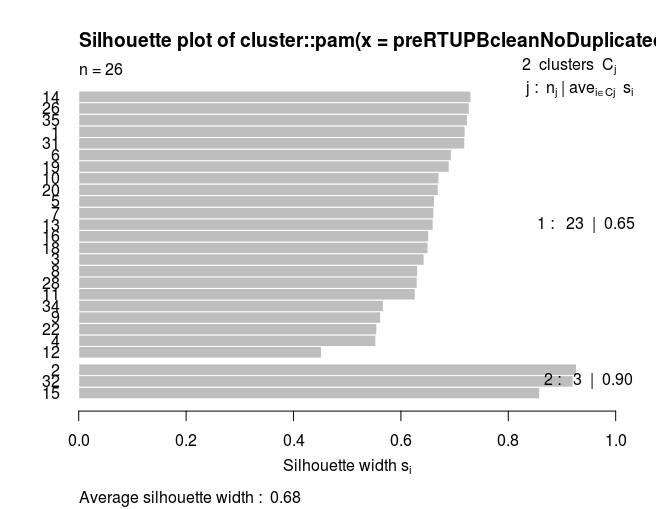
\includegraphics[width=0.75\textwidth]{../Fig/RTUPB/rtupb-sil-k2-pre}
\caption{Moyenne silouhette }
\end{figure}



\begin{figure}[H]
\centering
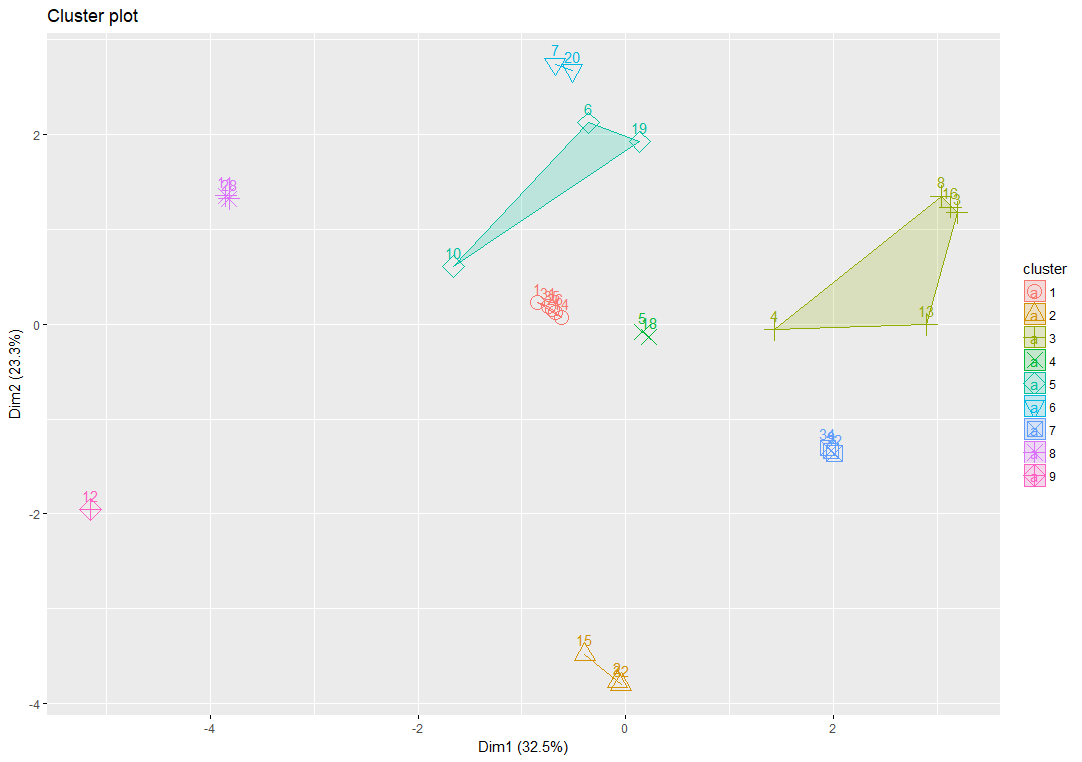
\includegraphics[width=0.90\textwidth]{../Fig/RTUPB/rtupb-pam-k9.png}
\caption{Nuage de point resultant de PAM k=9 }
\end{figure}

\begin{figure}[H]
\centering
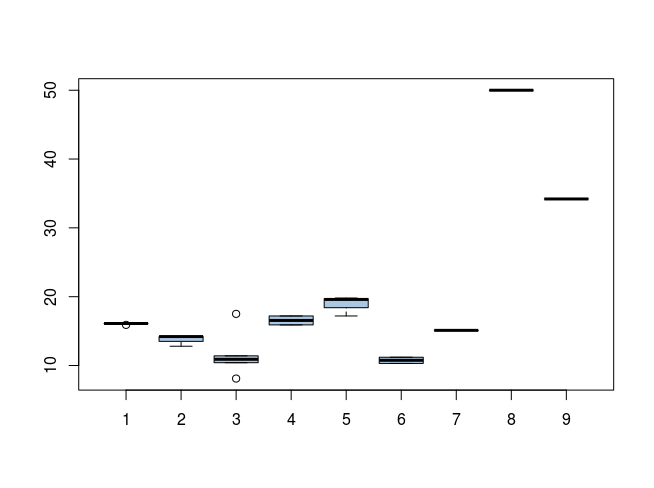
\includegraphics[width=0.90\textwidth]{../Fig/RTUPB/rtupb-qmax-k9-distribution}
\caption{Distribution QMAX  12mois  k=9 }
\end{figure}







%\begin{figure}[h]
%    \begin{minipage}[c]{.46\linewidth}
%        \centering
%        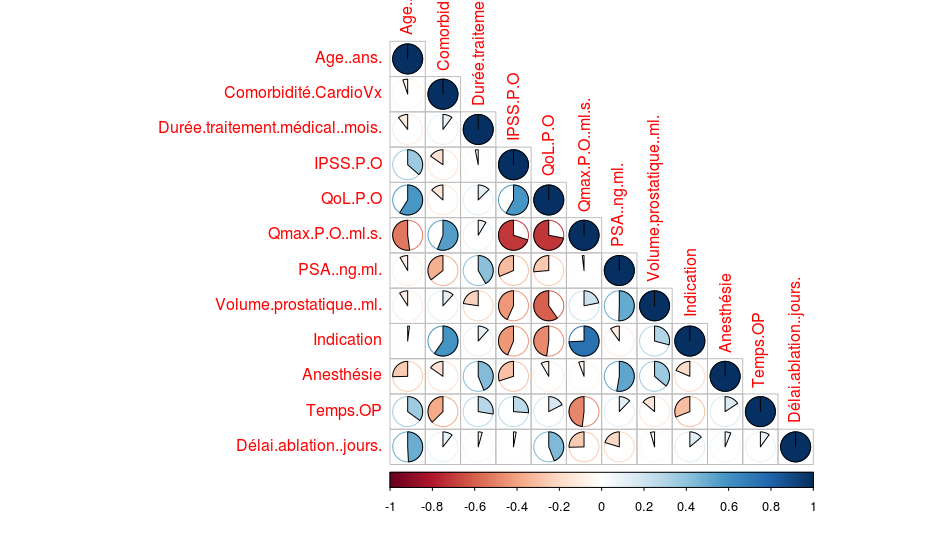
\includegraphics[width=1\textwidth]{../Fig/VPPBS/vppbs-corr-matrice-pie}
%        \caption{Légende}
%    \end{minipage}
%    \hfill%
%    \begin{minipage}[c]{.46\linewidth}
%        \centering
%        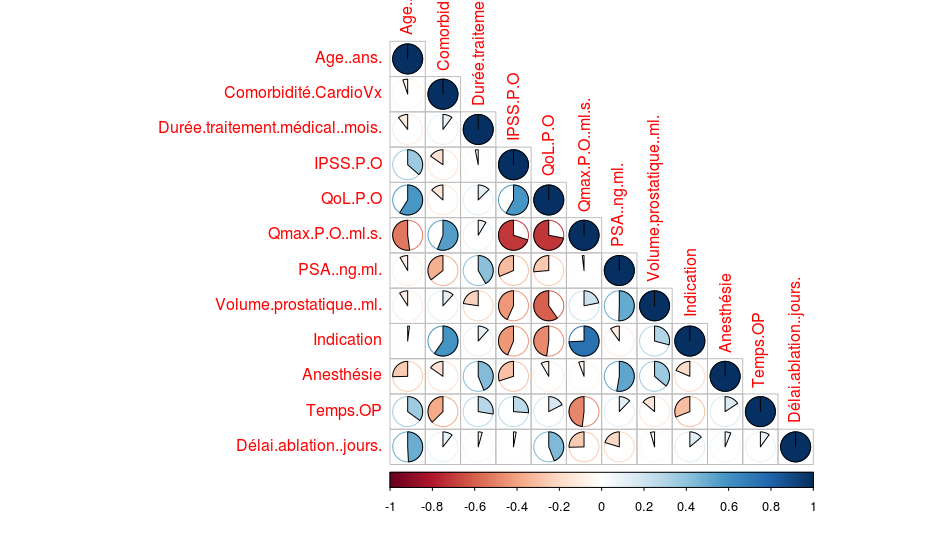
\includegraphics[width=1\textwidth]{../Fig/VPPBS/vppbs-corr-matrice-pie}
%        \caption{Légende}
%    \end{minipage}
%\end{figure}





%
%##########################
%# CONCLUSION
%##########################